\documentclass{beamer}
\usetheme{Madrid} % My favorite!
\usepackage{colortbl}
\usepackage{amsmath}
\usepackage{color}
\usepackage{textpos}
\setlength{\TPHorizModule}{1cm} % Horizontale Einheit
\setlength{\TPVertModule}{1cm} % Vertikale Einheit
%\usetheme{Boadilla} % Pretty neat, soft color.
%\usetheme{default}
%\usetheme{Warsaw}
%\usetheme{Bergen} % This template has nagivation on the left
%\usetheme{Frankfurt} % Similar to the default 
%with an extra region at the top.
%\usecolortheme{seahorse} % Simple and clean template
%\usetheme{Darmstadt} % not so good
% Uncomment the following line if you want %
% page numbers and using Warsaw theme%
% \setbeamertemplate{footline}[page number]
%\setbeamercovered{transparent}
%\setbeamercovered{invisible}
% To remove the navigation symbols from 
% the bottom of slides%
\usepackage[T1]{fontenc}
\setbeamertemplate{navigation symbols}{} 
\setbeamertemplate{itemize items}[default]
\usefonttheme[onlymath]{serif}
%\usepackage{biblatex}
\usepackage{graphicx}
\usepackage{sidecap}
\usepackage{setspace}
\newcommand\smallfont{\fontsize{6}{2}\selectfont}
\bibliography{/usr/local/texlive/texmf-local/bibtex/bib/local/library}
%\usepackage{bm}         % For typesetting bold math (not \mathbold)
%\logo{\includegraphics[height=0.6cm]{yourlogo.eps}}
%


\include{slide-macros}

\title[Two applications of simple allele frequency models]{Allele frequency models}
\author{Graham Coop}
\institute[UCD]
{
University of California, Davis \\
$@\textrm{graham\_coop}$\\
www.gcbias.org\\
}
\date{\today}
%will show current date. 
% Alternatively, you can specify a date.
%
\begin{document}

\begin{frame}
\titlepage
\end{frame}

% \begin{frame}{Introduction}


% \end{frame}

\begin{frame}{Two vaguely related projects}
\begin{columns}
\begin{column}{0.5\textwidth}
Isolation by Distance.
	\begin{center} 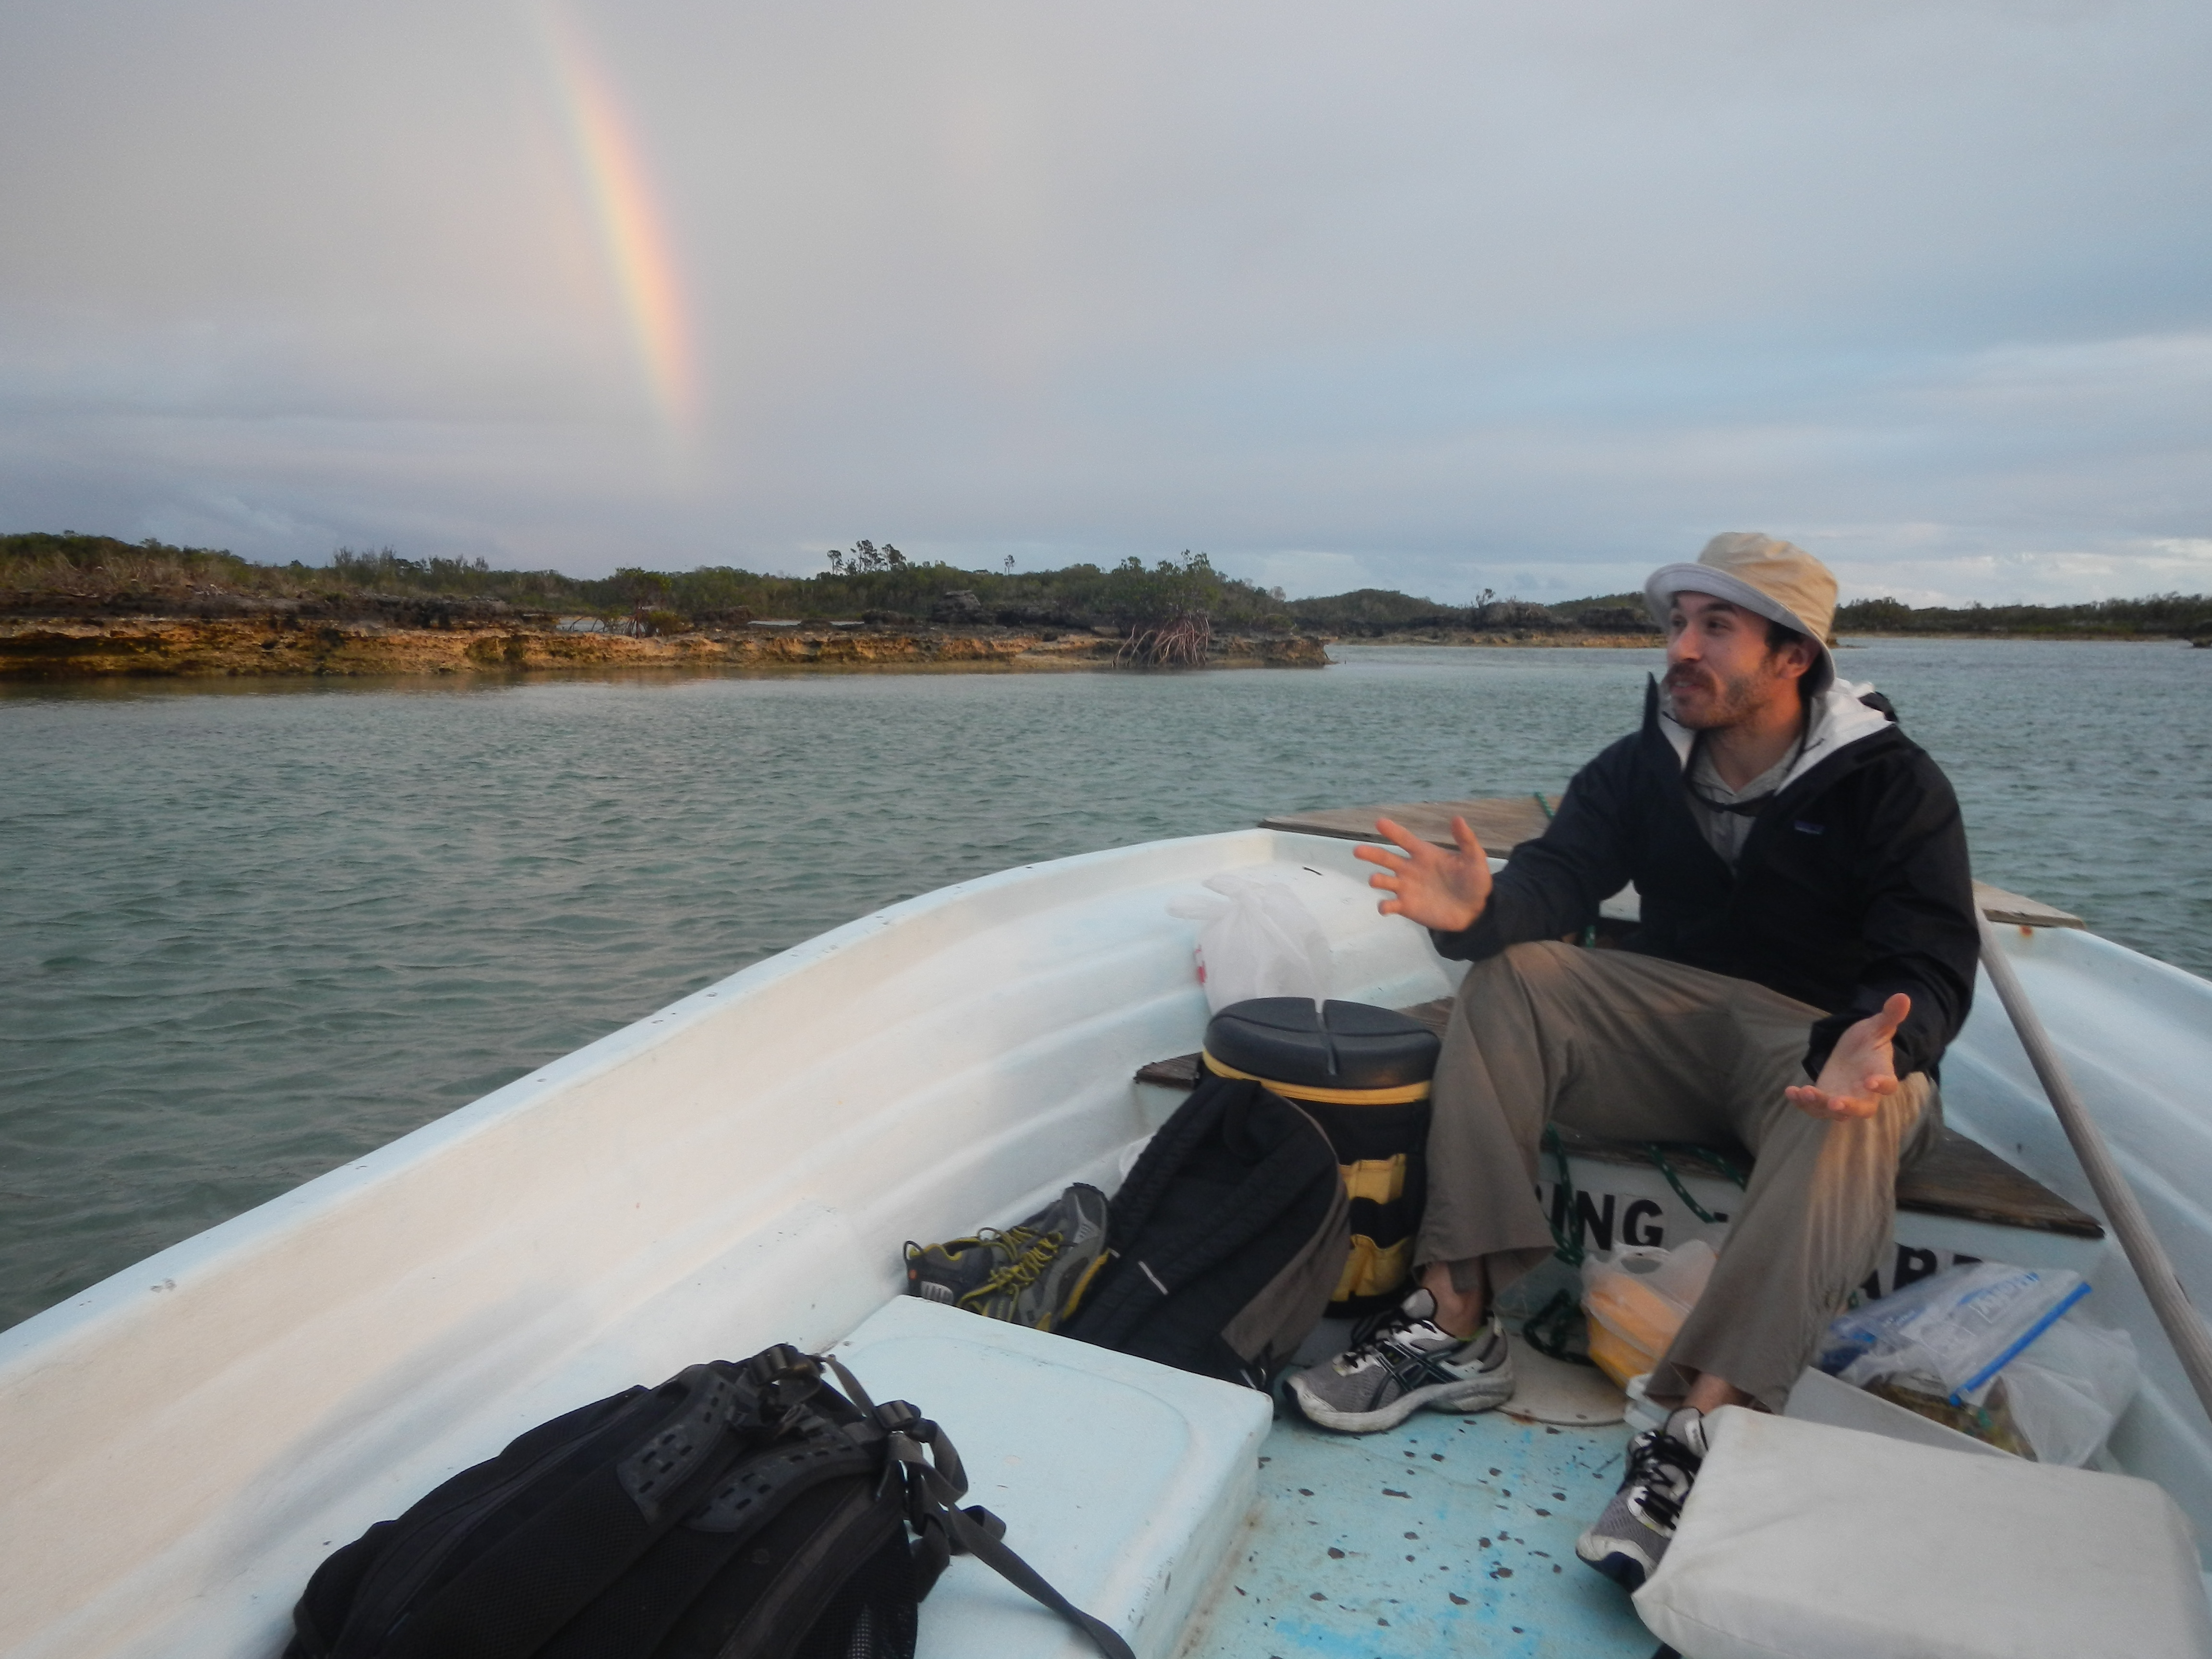
\includegraphics[width=0.7
          \textwidth]{../figs/Gideon}       \end{center} 
	\vskip -0.5cm
 {\tiny          Gideon Bradburd }

     \begin{center}
         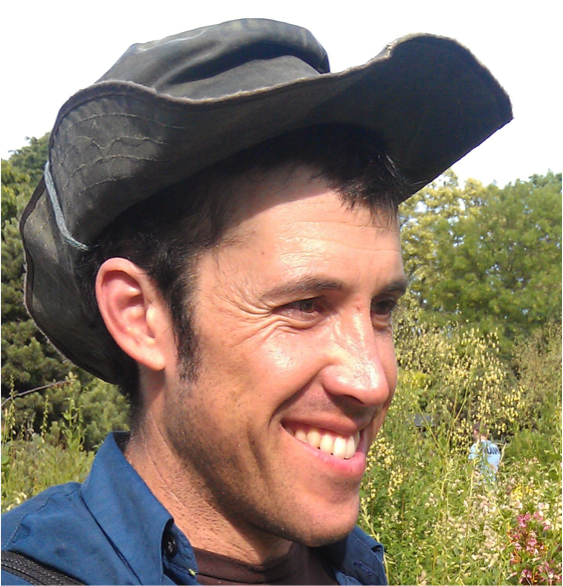
\includegraphics[width=0.3 \textwidth]{../figs/Peter_Ralph.png}
      \end{center}
	\vskip -0.5cm
 {\tiny          Peter Ralph }

\end{column}
\begin{column}{0.5\textwidth}
\pause 
The signal of polygenic adaptation\\
	\begin{center} \includegraphics[width=0.7
          \textwidth]{../figs/Jeremy_Berg} \end{center}

\end{column}
\end{columns}
\end{frame}


\begin{frame}
	\frametitle	{The Expected Distribution Under Neutrality}
	\begin{columns}
		\begin{column}{0.3 \textwidth}
			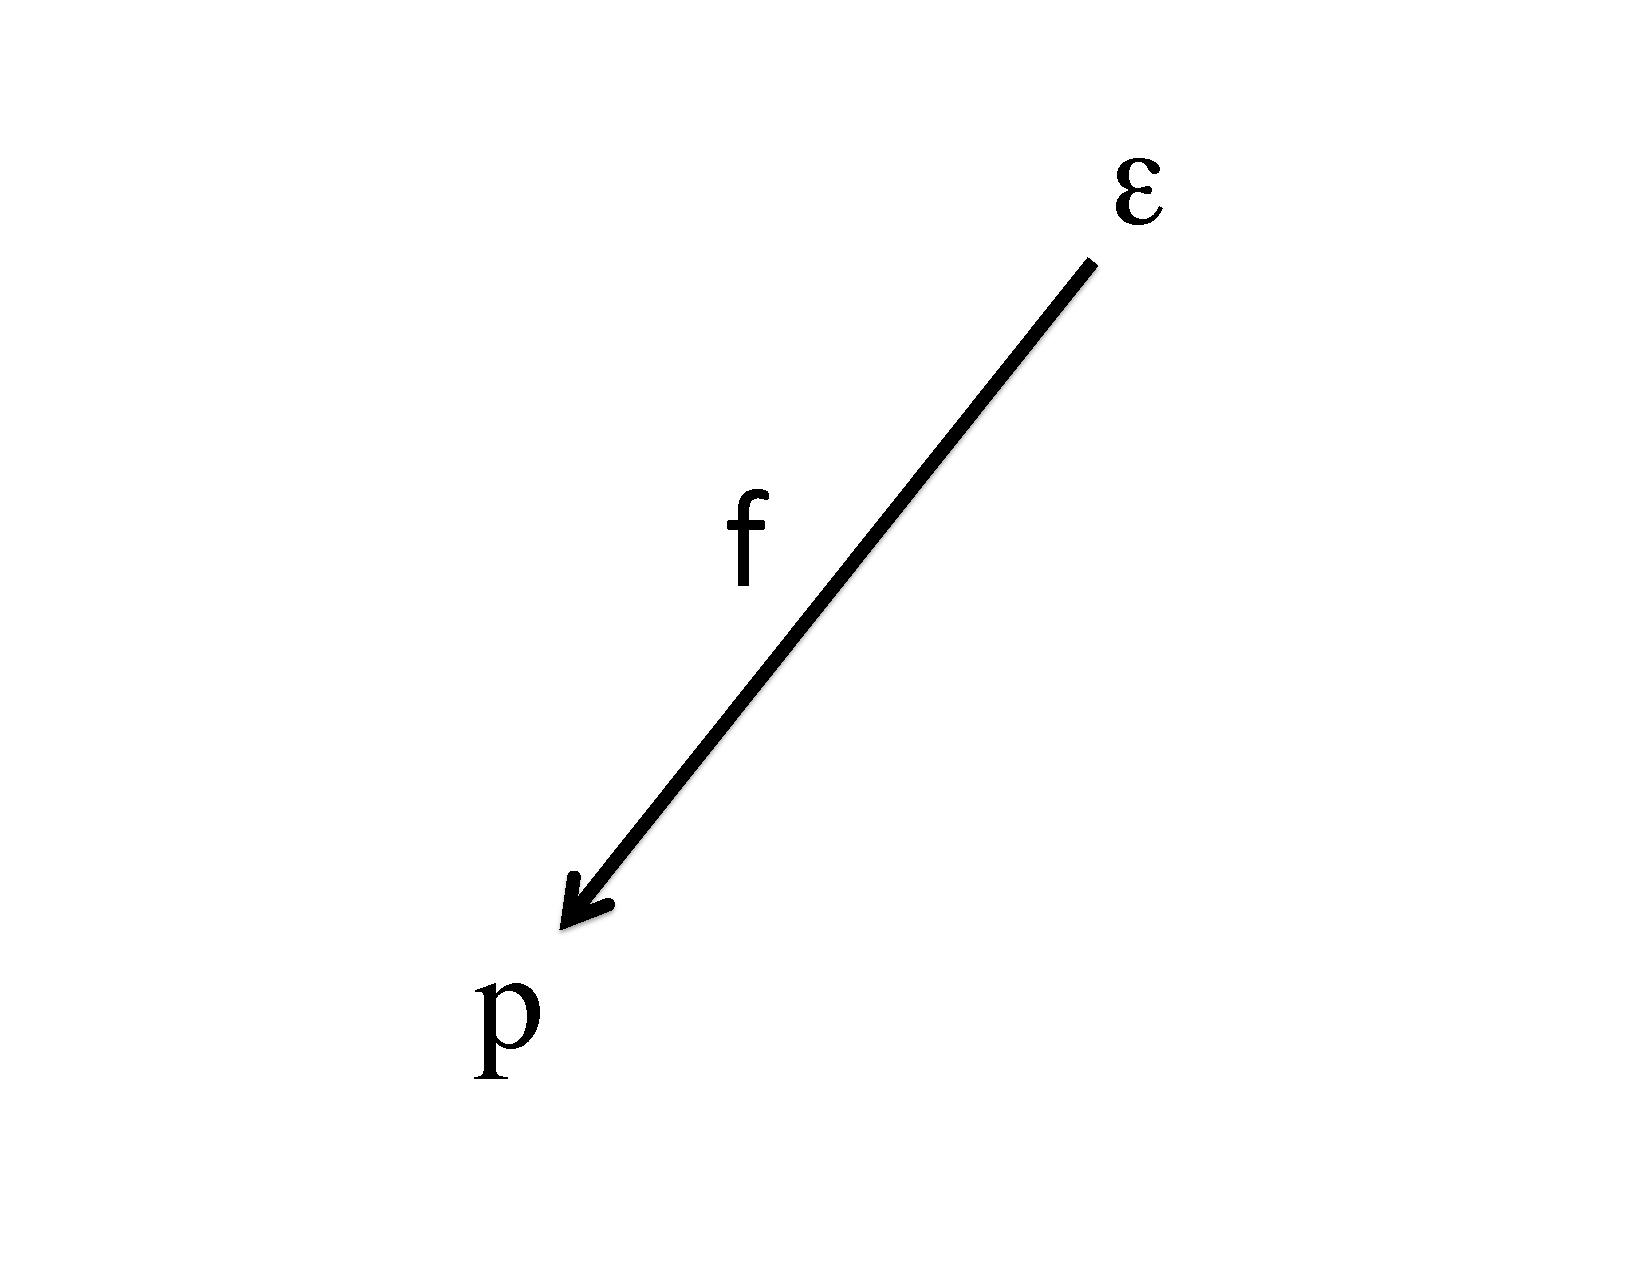
\includegraphics[height =
                        \textwidth]{../figs/OneBranch.pdf}
%			\only<2>{\includegraphics[height = \textheight]{../figs/TwoBranch.pdf}}
%			\only<2-3>{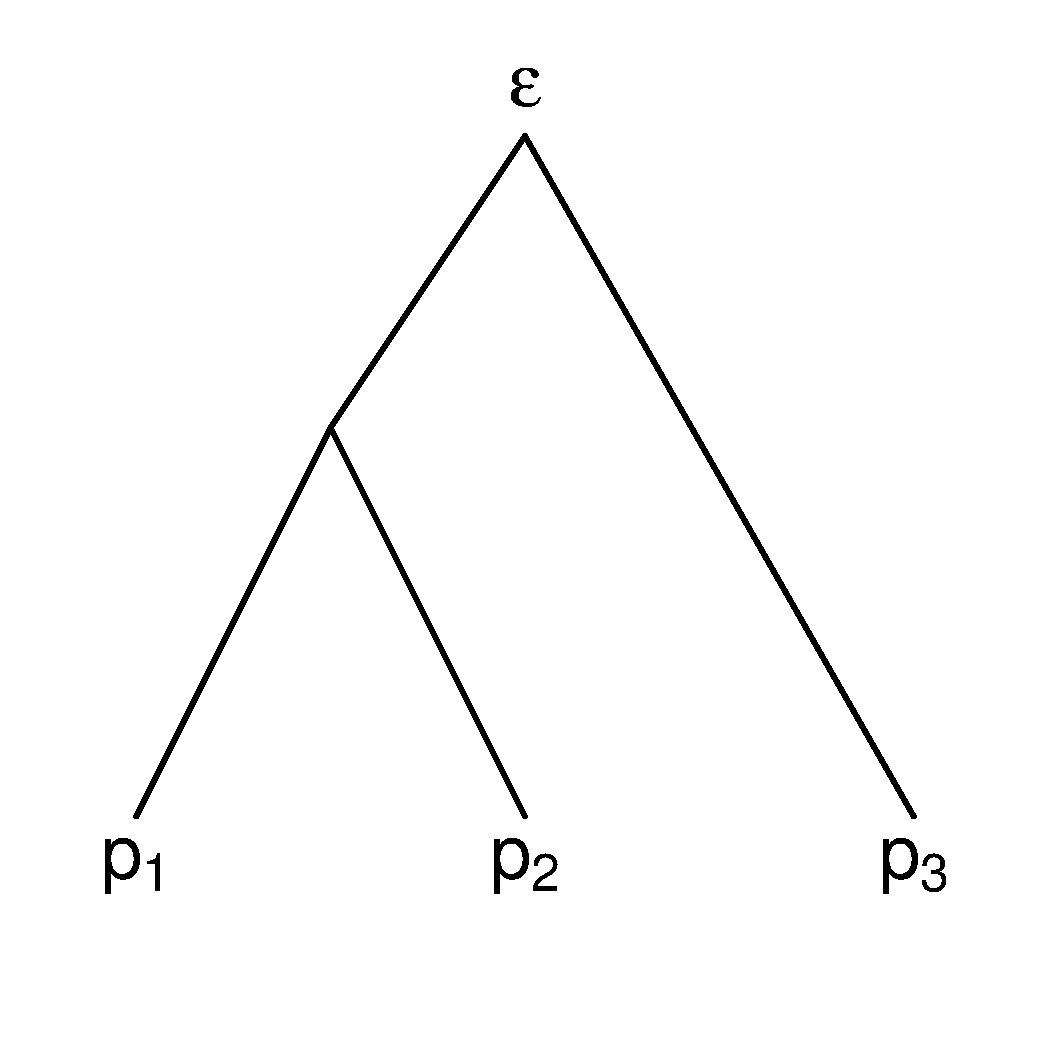
\includegraphics[height = \textheight]{../figs/ThreeBranch.pdf}}

					\begin{block}{The Normal Model}
						$\mathbb{E}\left[p\right] = \epsilon$ \\
						\vskip 0.4cm
						$\mathbb{V}\left[p\right] = f \epsilon ( 1 - \epsilon )$
					\end{block}

		\end{column}
		\begin{column}{0.45\textwidth}

			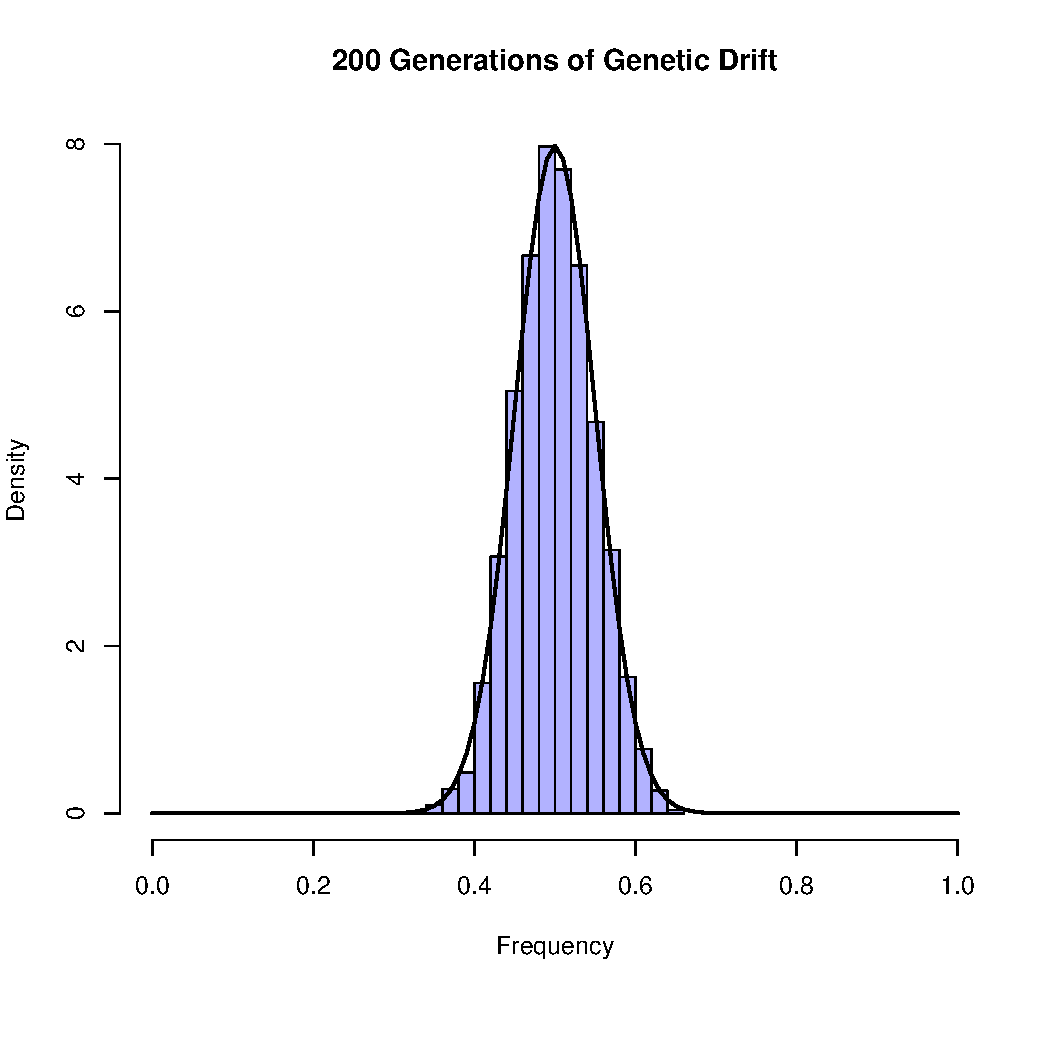
\includegraphics[width = 1.5 \textwidth]{../figs/Hist200gens.pdf}
					
		\end{column}
	\end{columns}
\end{frame}

\begin{frame}
	\frametitle	{The Expected Distribution Under Neutrality}
	\begin{columns}

		\begin{column}{0.56\textwidth}
                  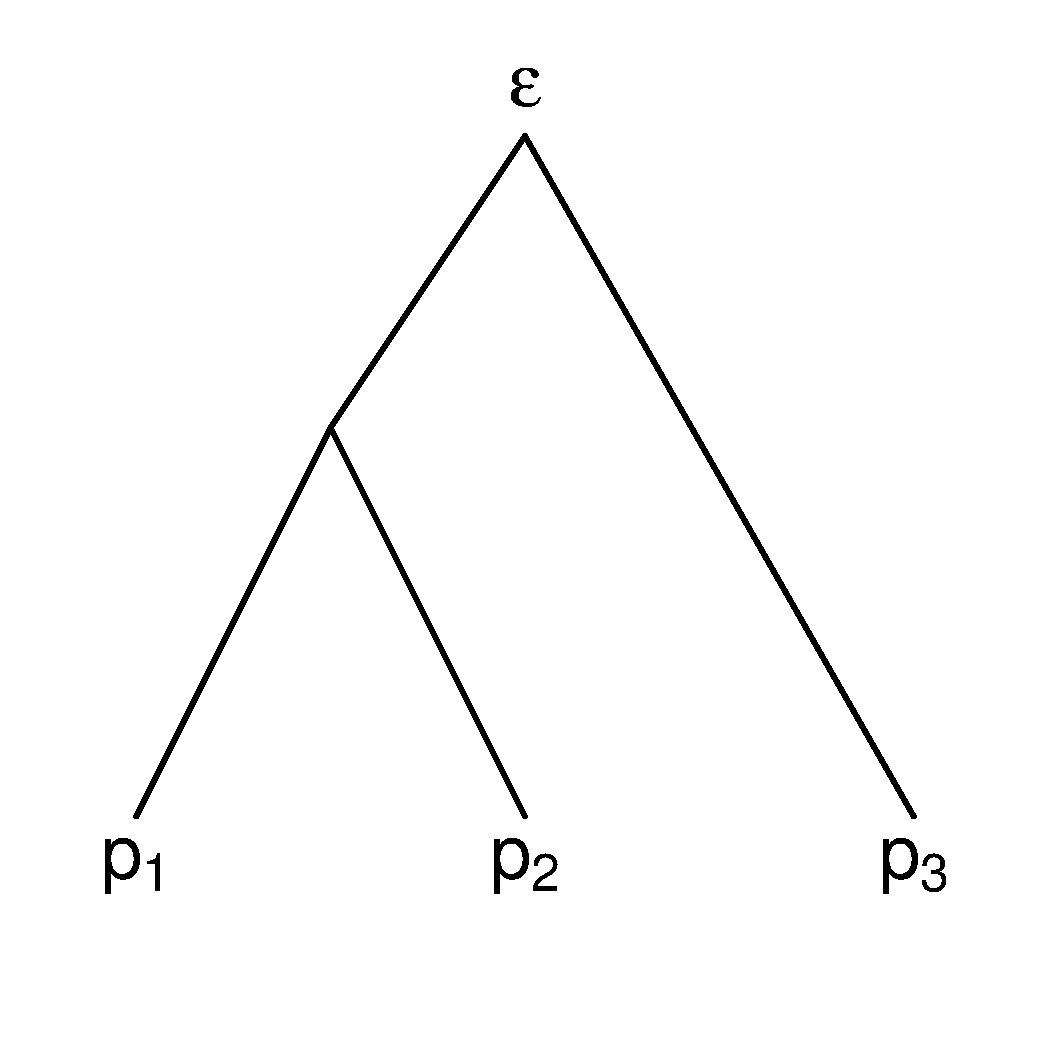
\includegraphics[height = \textheight]{../figs/ThreeBranch.pdf}
		\end{column}

		\begin{column}{0.45\textwidth}


		%	\only<2>{\vskip-5.9cm
		%			\begin{block}{The Multivariate Normal Model}
		%				$\mathbb{E}\left[\vec{p}\ \right] = \epsilon$ \\
		%				\vskip 0.4cm
		%				$\mathbb{V}\left[\vec{p}\ \right] = \epsilon ( 1 - \epsilon ) \begin{bmatrix}f_{11}&f_{12}\\f_{21}&f_{22}\end{bmatrix}$
		%			\end{block}
		%			}
		\only<1-2>{\vskip-5.9cm
					\begin{block}{The Multivariate Normal Model}
						$\mathbb{E}\left[\vec{p}\ \right] = \epsilon$ \\
						\vskip 0.4cm
						$\mathbb{V}\left[\vec{p}\ \right] = \epsilon ( 1 - \epsilon ) \begin{bmatrix}f_{11}&f_{12}&0\\f_{21}&f_{22}&0\\0&0&f_{33}\end{bmatrix}$
					\end{block}
					}
{\tiny Cavalli-Sforza \& Edwards. (1967) }
		\end{column}
	\end{columns}
\end{frame}


\begin{frame}{Population Structure}
\pause
	\begin{center} \includegraphics[width= 0.5 \textwidth]{../smbe_spacemix_figs/tree_mix}
\end{center}

\end{frame}


\begin{frame}{Isolation by distance datasets}
\pause
\begin{columns}
\begin{column}{0.4\textwidth}

	\begin{center} 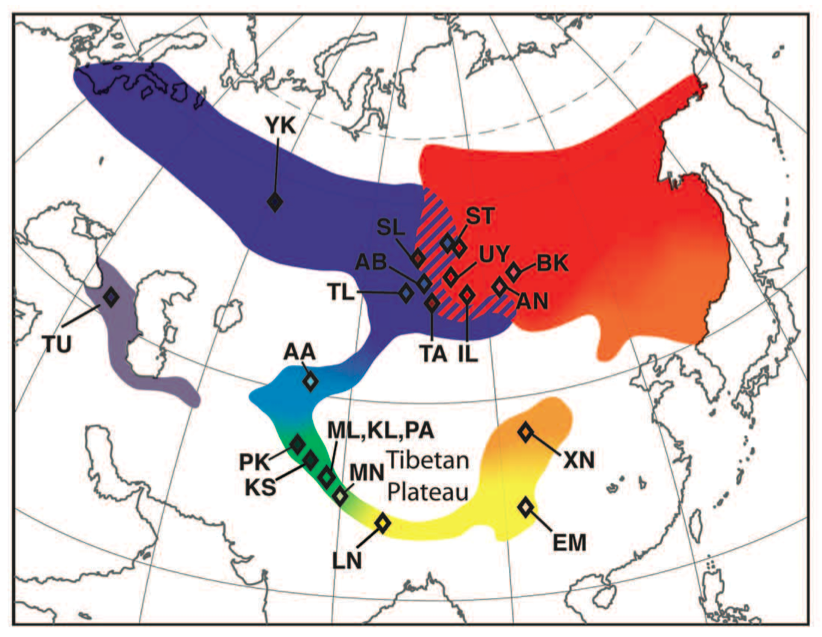
\includegraphics[width=
          0.8
          \textwidth]{../smbe_spacemix_figs/Irwin_warbler_map_figure}
\end{center}
	\vskip -0.5cm
          {\tiny Alcaide et al. (2014) Nature} 
\end{column}
\begin{column}{0.6\textwidth}
\pause 

	\begin{center} 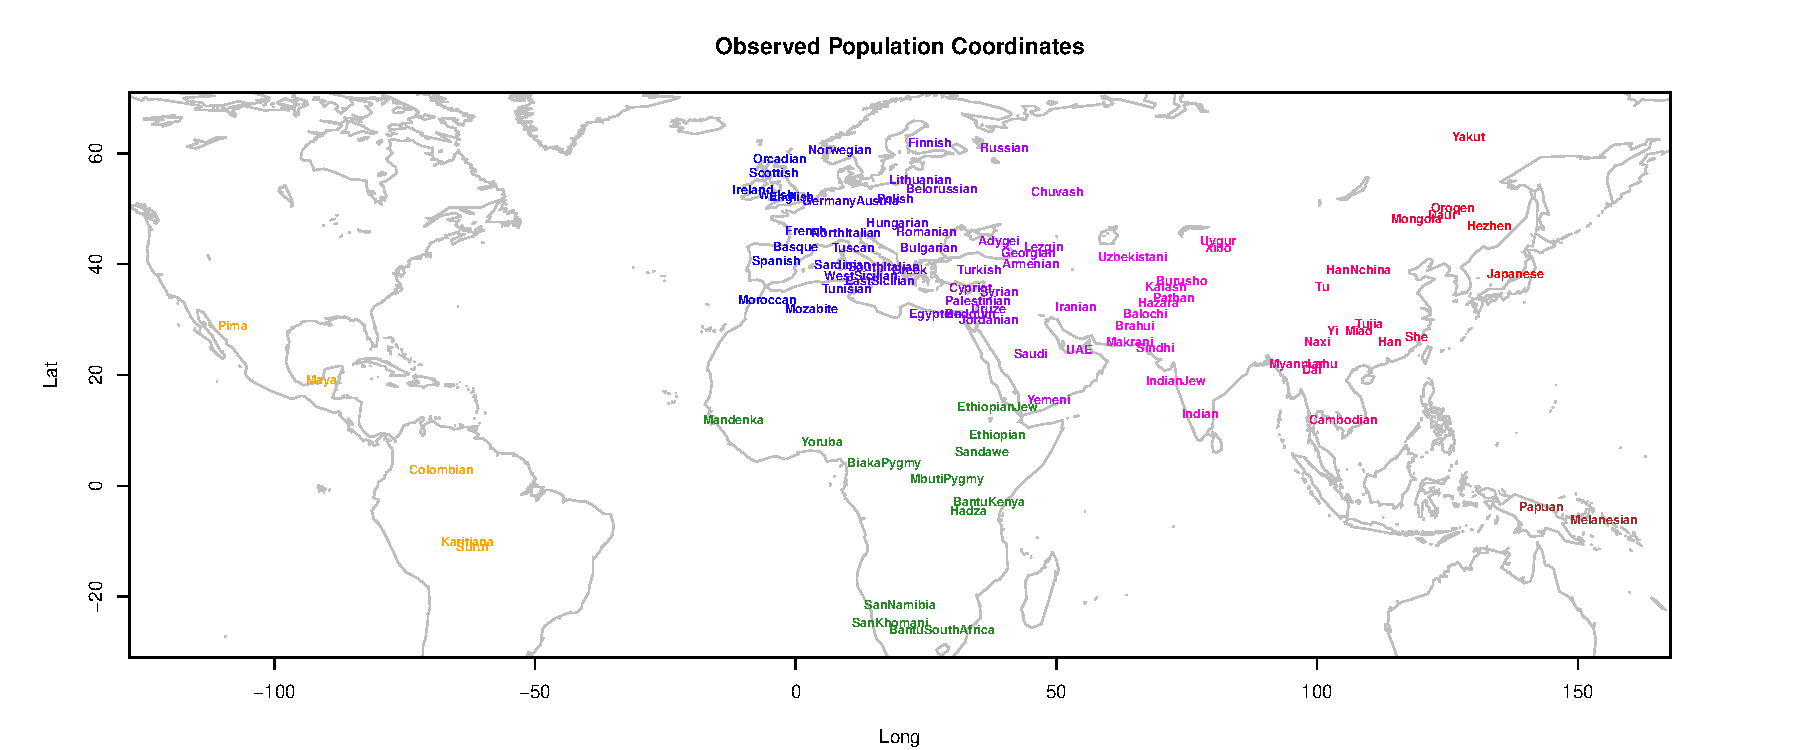
\includegraphics[width= 1.1 \textwidth, height = 0.6 \textheight]{../smbe_spacemix_figs/globe_obs_map_option2}
 \end{center}
          {\tiny Hellenthal et al. (2014) Science.}  
\end{column}
\end{columns}
\end{frame}

\begin{frame}
\frametitle{Isolation by distance}
{\small Covariance in allele freq (f) between i \& j around mean $\epsilon$  =
$ \hat{F}_{ij} = \frac{1}{L} \sum_{l=1}^L (f_{il} -
\epsilon_l)(f_{jl}-\epsilon_l) $ }
	\vskip -0.5cm
	\begin{center} 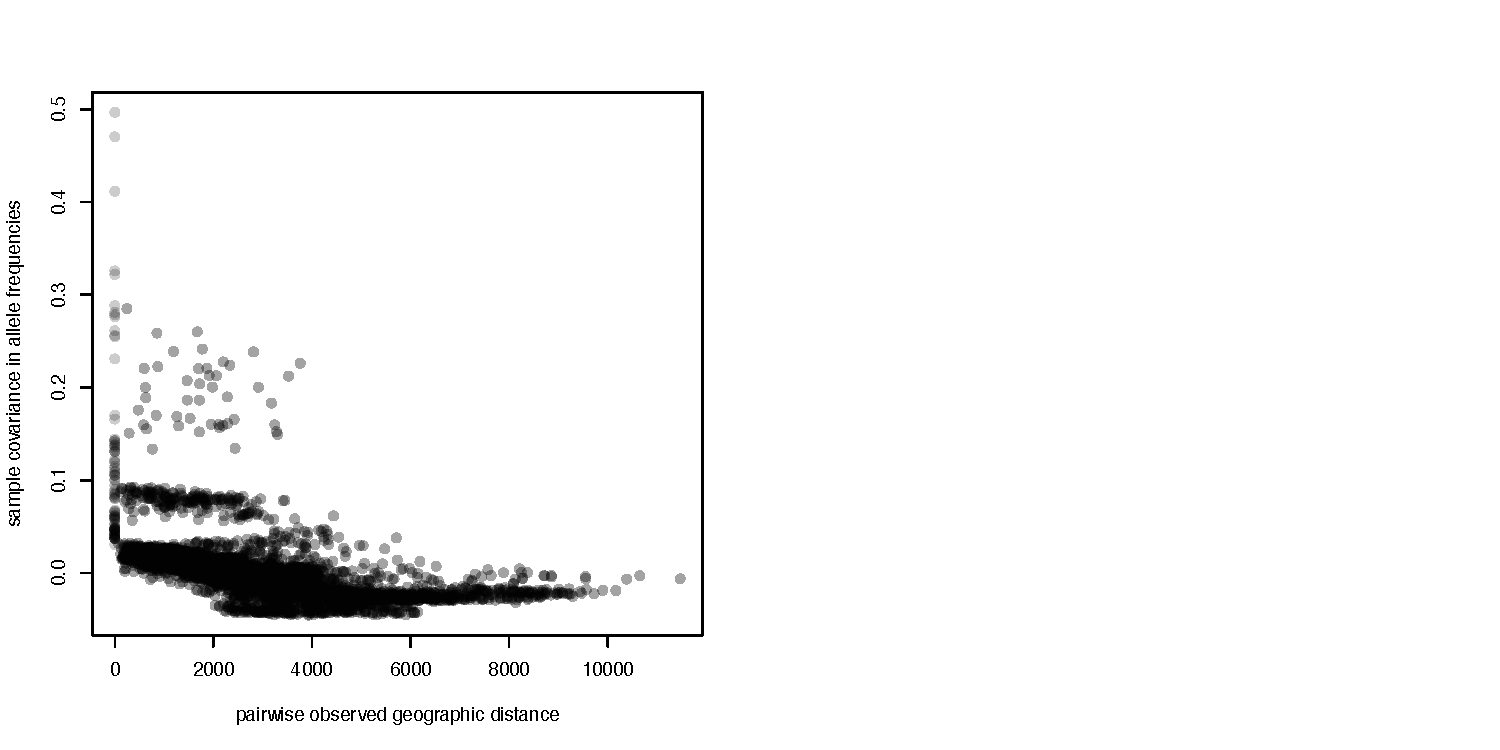
\includegraphics[width= 0.6 \textwidth]{../smbe_spacemix_figs/cropped_globe_sampleV} \end{center}
\end{frame}

\begin{frame}
\frametitle{Isolation by distance}
Parametric approximation {\small ${F}_{ij} = \frac{1}{\alpha_0} \exp \left(
  -\alpha_1 D_{ij}^{\alpha_2} \right) + \color{blue}{ \delta_{ij} \beta_i }$} 
	\vskip -0.5cm
	\begin{center} 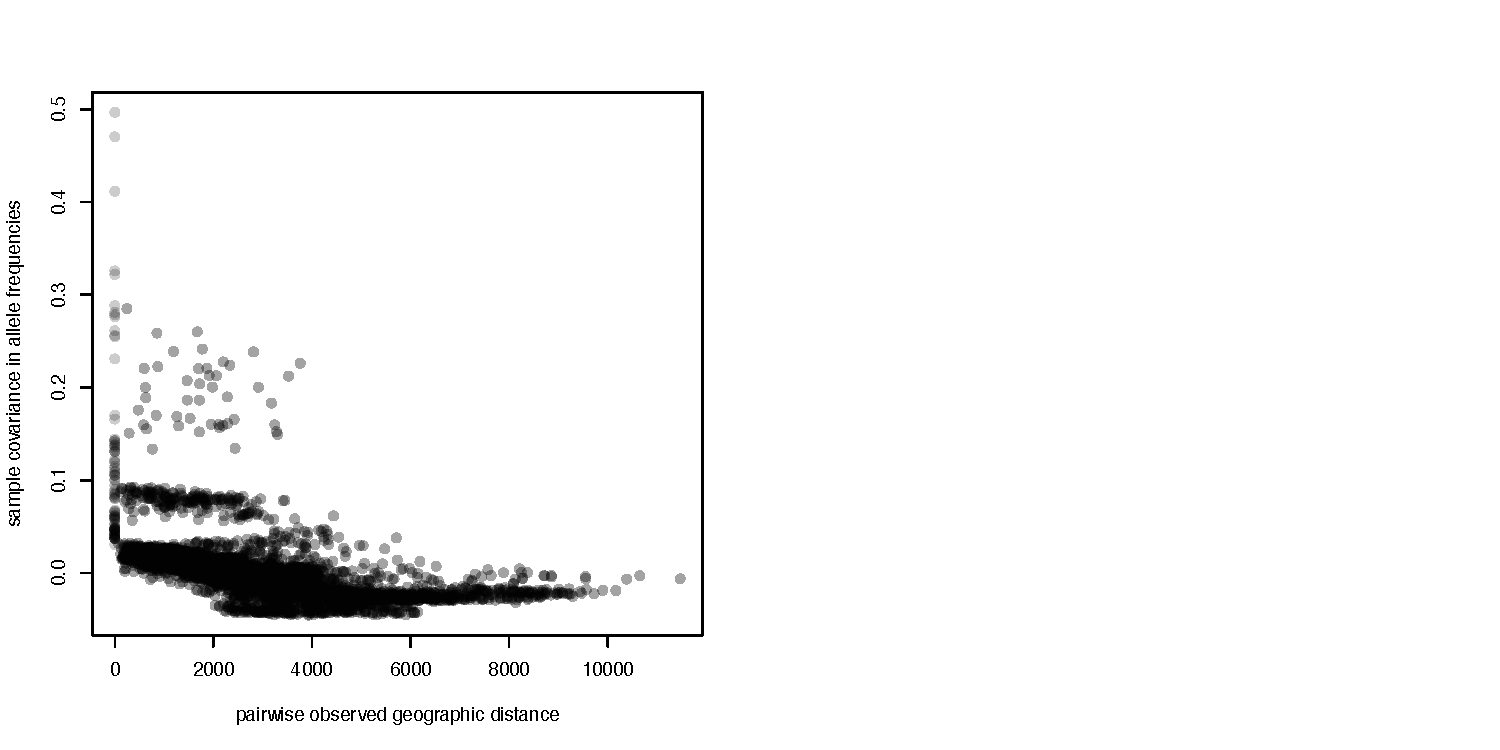
\includegraphics[width=  0.6 \textwidth]{../smbe_spacemix_figs/cropped_globe_sampleV} \end{center}
\end{frame}


\begin{frame}
\frametitle{Isolation by distance}
Obs. covariance in allele freq (f) between i \& j around mean $\epsilon$
\begin{equation*}
\hat{F}_{ij} = \frac{1}{L} \sum_{l=1}^L (f_{il} - \epsilon_l)(f_{jl}-\epsilon_l)
\end{equation*}
Exp. covariance between i \& j
\begin{equation*}
{F}_{ij} = \frac{1}{\alpha_0} \exp \left( -\alpha_1 D_{ij}^{\alpha_2} \right)
\end{equation*}
So the likelihood of our covariance matrix
\begin{equation*}
P \big(\hat{F} | F(D,\vec{\alpha}), L \big) \sim W(F,L)
\end{equation*}
Put priors on params., do MCMC.
\end{frame}

\begin{frame}
\frametitle{Isolation by distance in Humans}
	\begin{center} 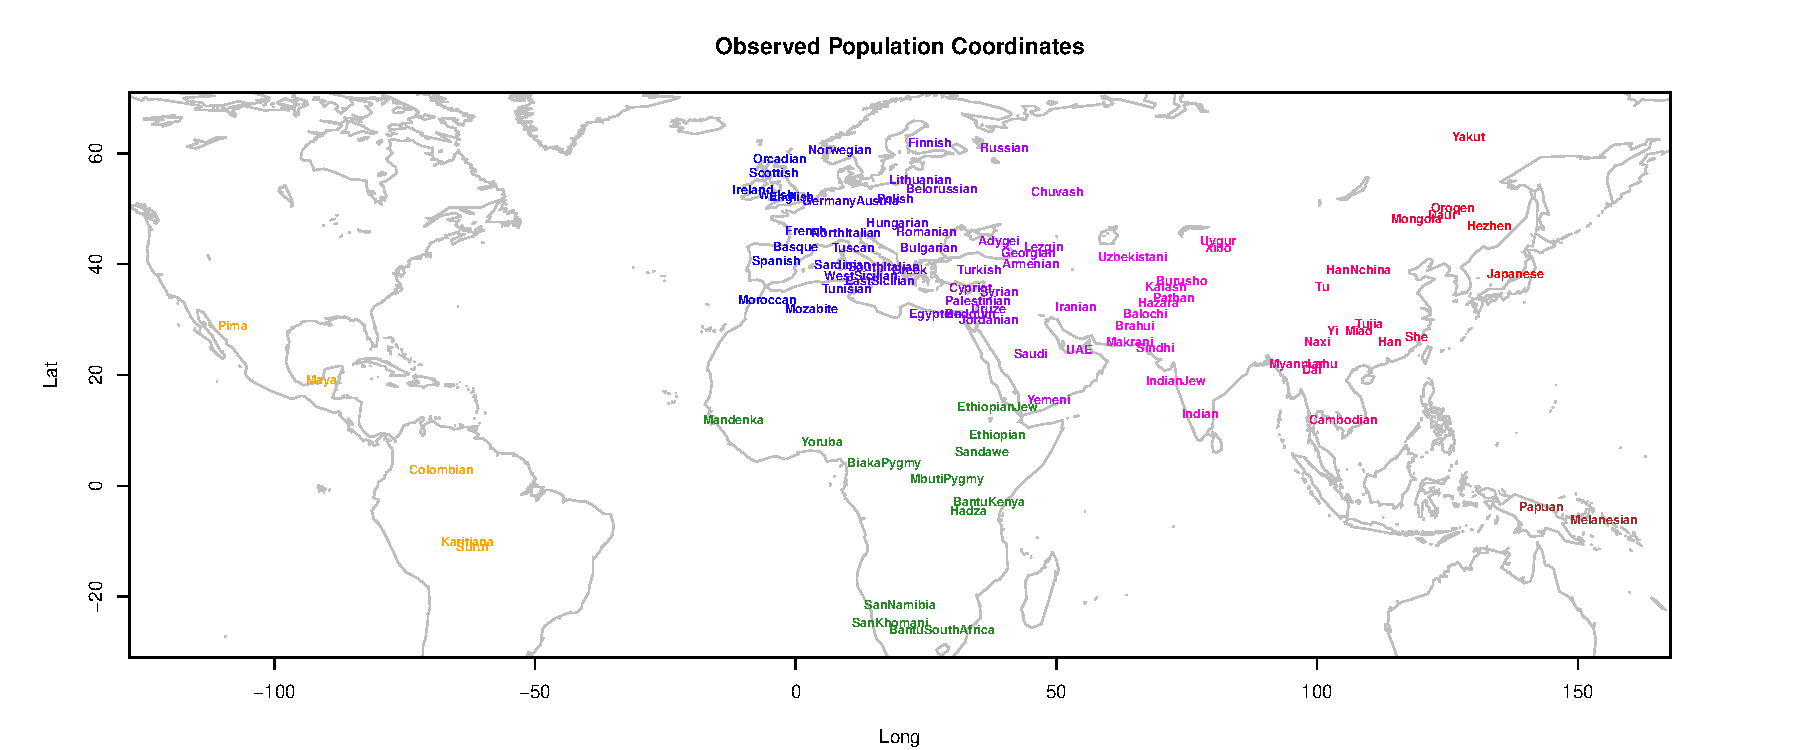
\includegraphics[width=\textwidth]{../smbe_spacemix_figs/globe_obs_map_option2}
 \end{center}
     {\tiny Hellenthal et al. (2014) Science.}  
\end{frame}

\begin{frame}
\frametitle{Isolation by distance in Humans}
	\begin{center} 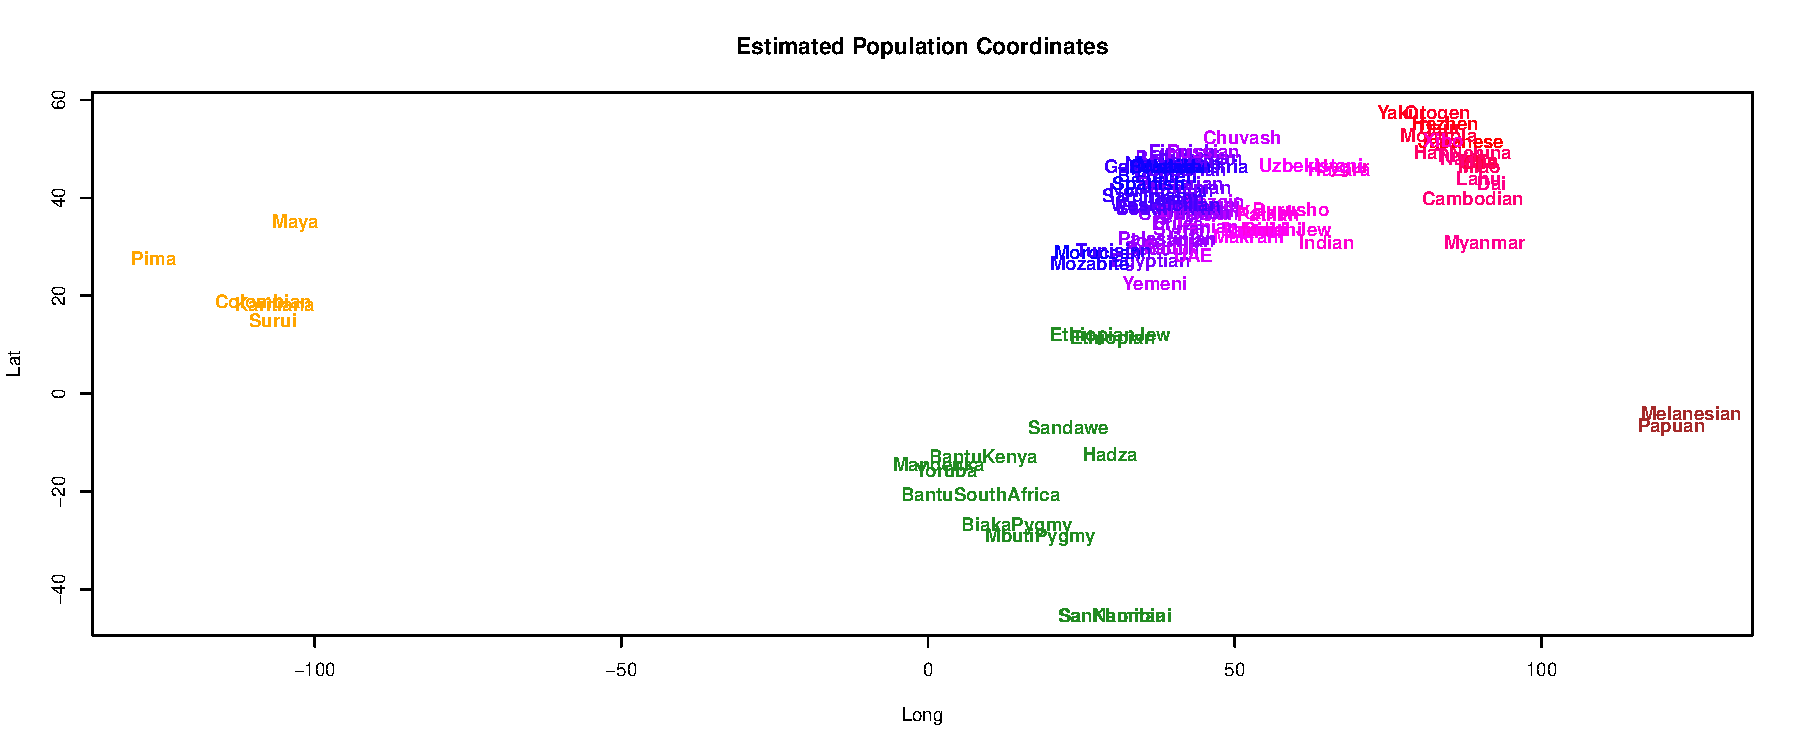
\includegraphics[width=\textwidth]{../smbe_spacemix_figs/globe_est_map}
 \end{center}
\end{frame}

\begin{frame}
\frametitle{Isolation by distance in Humans}
	\begin{center} \includegraphics[width= \textwidth]{../smbe_spacemix_figs/globe_est_map_eurasia2}
 \end{center}
\end{frame}

\begin{frame}
\frametitle{Isolation by distance in Humans}
	\begin{center} \includegraphics[width= \textwidth]{../smbe_spacemix_figs/globe_est_map_eurasia2}
 \end{center}
\end{frame}

\begin{frame}{Isolation by distance in Greenish Warblers}

\begin{columns}
\begin{column}{0.4\textwidth}

	\begin{center} 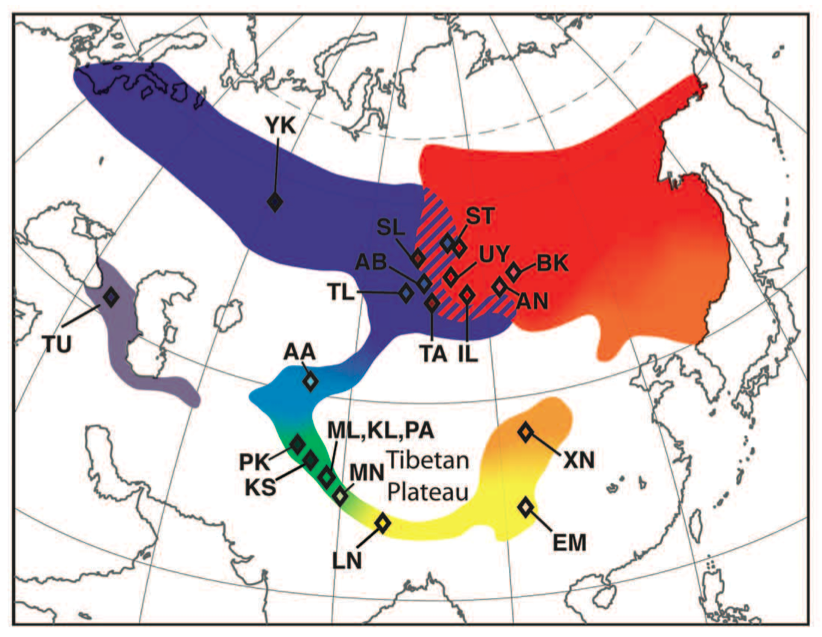
\includegraphics[width=\textwidth]{../smbe_spacemix_figs/Irwin_warbler_map_figure}
\end{center}
	\vskip -0.5cm
          {\tiny Alcaide et al. (2014) Nature} 
\end{column}
\begin{column}{0.6\textwidth}
\pause 

	\begin{center} \includegraphics[width= \textwidth]{../smbe_spacemix_figs/warbler_est_map}
 \end{center}
\end{column}
\end{columns}
\end{frame}

\begin{frame}{Isolation by distance in Greenish Warblers}

\begin{columns}
\begin{column}{0.4\textwidth}

	\begin{center} \includegraphics[width= \textwidth]{../smbe_spacemix_figs/warbler_est_map}
\end{center}
	\vskip -0.5cm
          {\tiny Alcaide et al. (2014) Nature} 
\end{column}
\begin{column}{0.6\textwidth}
\pause 

	\begin{center} \includegraphics[width=\textwidth]{../smbe_spacemix_figs/warbler_est_map_contactzone2}
 \end{center}
\end{column}
\end{columns}
\end{frame}

\begin{frame}{Violations of Isolation by distance in Greenish Warblers}

\begin{columns}
\begin{column}{0.4\textwidth}
We can predict allele freq. at locus $l$ at pop. $i$'s location given all neighbours $\mu_{i,l}$
\begin{equation*}
\textrm{F-stat}_{i,j}  = \frac{1}{L} \sum_{l=1}^L  (f_{il} - \mu_{i,l} )(f_{jl}-\epsilon_l)
\end{equation*}
Will be zero if model fits well. $j$ can be either another sampled
population or a location where we can predicted allele freq.
\end{column}
\begin{column}{0.6\textwidth}
\pause 

	\begin{center} 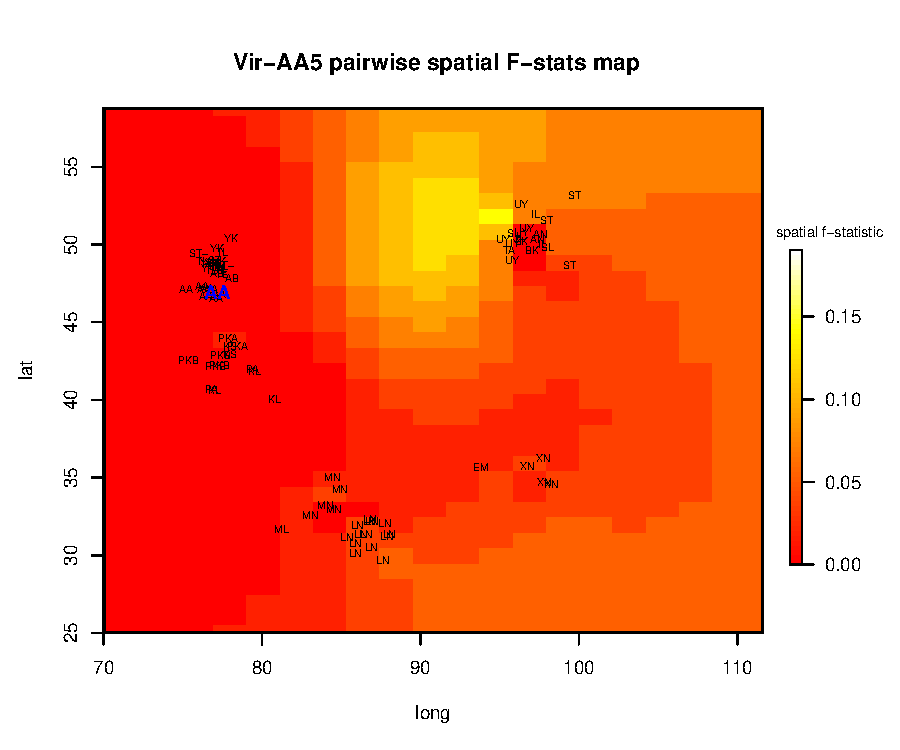
\includegraphics[width=  0.9 \textwidth]{../smbe_spacemix_figs/fstat_map_Vir-AA5}
 \end{center}
\end{column}
\end{columns}
\end{frame}


\begin{frame}{Fitting long distance admixture: Greenish Warblers}

\begin{columns}
\begin{column}{0.4\textwidth}
We can allow admixture from any spatial location in our model. We
allow population $i$ to draw $0<w_i<0.5$ of its ancestry from a
location $i'$. So the covar. between $i$ and $j$ becomes
\begin{align*}
F_{ij}^{\prime}  & = (1-w_i)(1-w_j) F(D_{ij})  \\
+ & w_i(1-w_j)F(D_{i'j})\\
+ & (1-w_i)w_j F(D_{ij'}) \\
+ & w_iw_j F(D_{i'j'})
\end{align*}
\end{column}
\begin{column}{0.6\textwidth}
\pause 

	\begin{center} 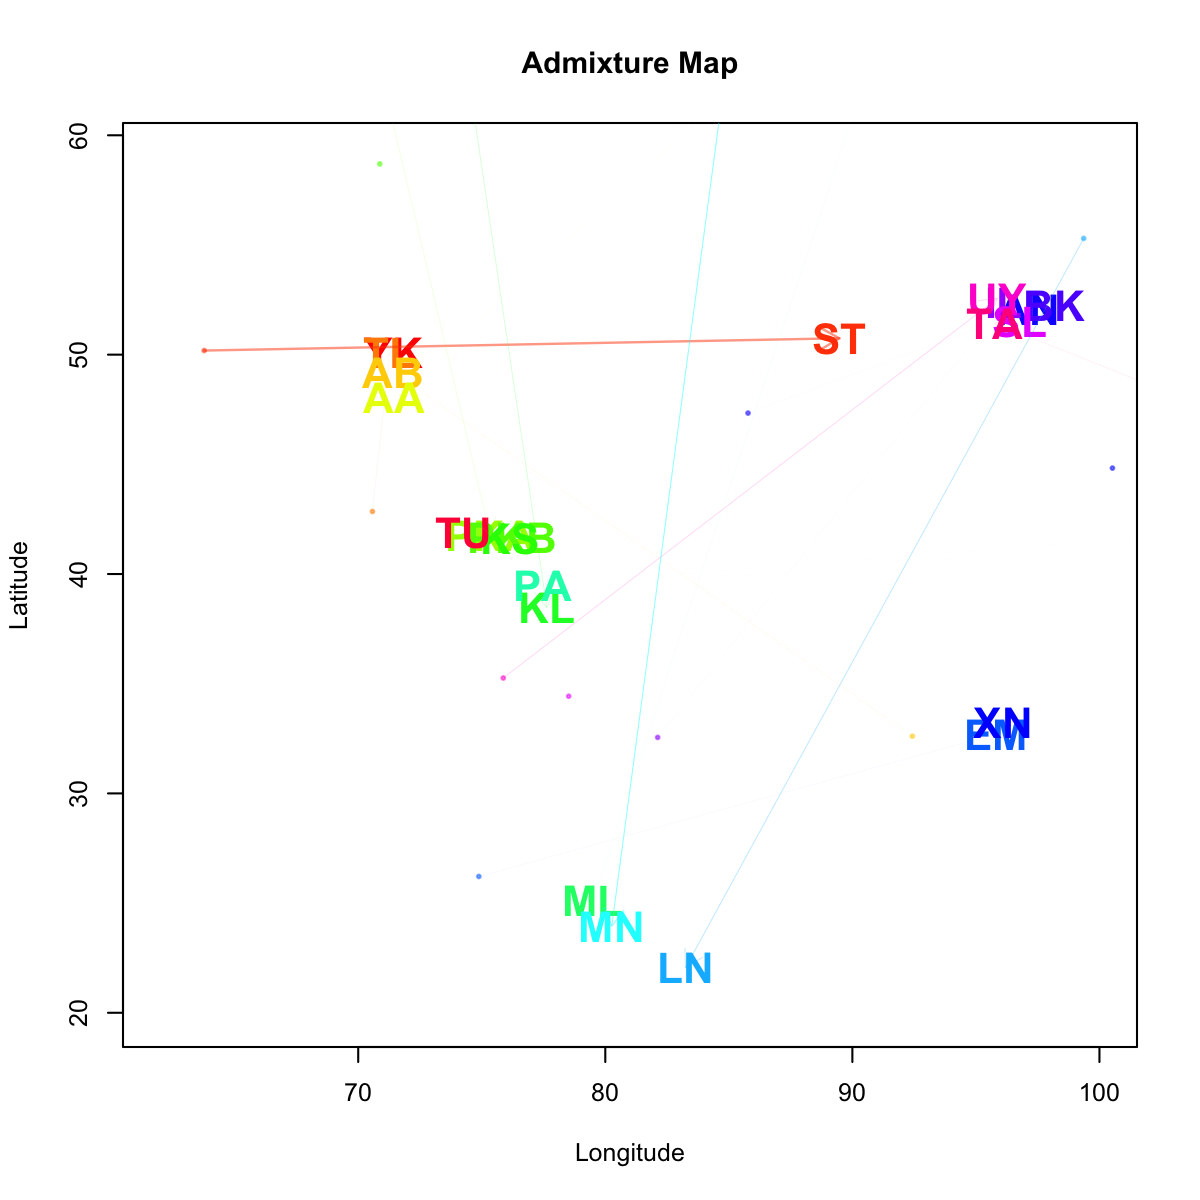
\includegraphics[width=  0.9 \textwidth]{../smbe_spacemix_figs/procrustes_warbler_admix_map_for_graham_talk}
 \end{center}
\end{column}
\end{columns}
\end{frame}


\begin{frame}{Extensions}

\end{frame}


\begin{frame}{Introduction}
\begin{columns}
\begin{column}{0.5\textwidth}
The signal of polygenic adaptation\\
	\begin{center} \includegraphics[width=0.7
          \textwidth]{../figs/Jeremy_Berg} \end{center}
\end{column}
\begin{column}{0.5\textwidth}
\pause 

	\begin{center} \includegraphics[width=
          \textwidth]{../figs/Berg_Coop_paper_title.png} \end{center}

	\begin{center} \includegraphics[width=
          \textwidth]{../figs/Haldanessieve.png} \end{center}

\end{column}
\end{columns}
\end{frame}


\begin{frame}
	\frametitle{Understanding Selection: Phenotypes first (Quant. Gen)}
			\begin{center} 	\includegraphics[scale =
                          0.35]{../figs/Darwins_Finches_example} \end{center}
			%\includegraphics[scale = 0.25]{../figs/CornExperiment}}
\end{frame}

\begin{frame}
	\frametitle{Understanding Selection: Genes First (Popgen)}
%Genes First (Population Genetics) \\
			\begin{center} \includegraphics[scale =
                          0.35]{../figs/SLC24A5_example} \end{center}
			%\includegraphics[scale = 0.25]{../figs/iHS1}
			%\includegraphics[scale = 0.28]{../figs/iHS2}
\end{frame}

% \begin{frame}
% 	\frametitle{Understanding Selection: Genes First (Popgen)}
% Environmental correlations (Coop et al 2010, Gunther and Coop 2013). 
% 			\begin{center} 
%                           \includegraphics[width=0.6 \textwidth]{../figs/example_corr_fig} 
%                         \end{center}

% \end{frame}

\begin{frame}
	\frametitle{Genome Wide Association Studies}
	\includegraphics[width = \textwidth]{../figs/Jostins} \\
	\includegraphics[width = \textwidth]{../figs/Morris} \\
	\includegraphics[width = \textwidth]{../figs/Speliotes}
\end{frame}


\begin{frame}
	\frametitle{Genome Wide Association Studies: BMI}
	\includegraphics[width = 0.9 \textwidth]{../figs/BMI_GWAS}
\end{frame}

\begin{frame}
	\frametitle{Genome Wide Association Studies}
	\includegraphics[width = \textwidth]{../figs/Atwell} \\
%	\includegraphics[width = \textwidth]{../figs/Jordan} \\
	\includegraphics[width = \textwidth]{../figs/Mackay}
\end{frame}

\begin{frame}
	\frametitle{Genome Wide Association Studies}
	\includegraphics[width = 0.9 \textwidth]{../figs/A_thaliana_GWAS}
\end{frame}


\begin{frame}
	\frametitle{What do we do with all of these loci?}

\end{frame}

\begin{frame}
	\frametitle{Using GWAS to construct additive genetic values}
	\begin{columns}
		\begin{column}{0.7\textwidth}
			\only<1>{\includegraphics[height = \textheight]{../figs/PlainEurope}}
			\only<2>{\includegraphics[height = \textheight]{../figs/PlainEuropeWOneArrow}}
			\only<3->{\includegraphics[height = \textheight]{../figs/PlainEuropeWTwoArrows}}
		\end{column}
		\begin{column}{0.3\textwidth}
			\only<2->{\begin{block}
						\only<2->{$\alpha = \text{effect size}$ \\}
						\only<3->{$p = \text{allele frequency}$ \\}
						\only<4>{$Z_m =$
                                                  constructed genetic value in pop $m$ \\
						\vspace{10pt}
						$Z_m = 2\sum_\ell \alpha_\ell p_{m\ell}$}
					\end{block}
					}
		\end{column}
	\end{columns}
\end{frame}

\begin{frame}
	\frametitle{Some Caveats}
These genetic values are far from predictive phenotypes for populations:
	\begin{itemize}
		\item We assume  additivity, i.e. no dominance or epistasis. 
		\item GWAS generally do not ascertain the causal mutation, but rather a SNP that is in linkage disequilibrium (LD) with it.
		\item Different populations experience different environments, which may alter phenotypes directly, or via gene by environment interactions
		\item We are missing a large number of variants
	\end{itemize}
	Nonetheless, these variants represent a rich, if partial, portrait of the genetic variation underlying phenotypic variation.
\end{frame}

\begin{frame}
	\frametitle{Worldwide Distribution of Constructed Height}
		\includegraphics[width = \textwidth]{../figs/LangoAllen} \\
		\includegraphics[width = \textwidth]{../figs/Turchin} \\
\end{frame}

\begin{frame}
	\frametitle{Distribution of Constructed Height in the HGDP}
	\includegraphics[width = \textwidth]{../figs/Height.pdf}
\end{frame}

\begin{frame}
	\frametitle{What About the Underlying Loci?}
	\includegraphics[width = \textwidth]{../figs/OneSNP.pdf}
\end{frame}




\begin{frame}
  \frametitle{Distribution of genetic values under neutrality}
\begin{block}{The Multivariate Normal Model}	
		\begin{columns}
		\begin{column}{0.5\textwidth}
		$\mathbf{F} = \begin{bmatrix}
							f_{11}&f_{12}&\dots& f_{1M} \\
							f_{21}&f_{22}&\dots& f_{2M} \\
							\vdots& \vdots& \ddots& \vdots \\
							f_{M1}& f_{M2}& \dots& f_{MM}
					\end{bmatrix}$
		\end{column}

		\begin{column}{0.5\textwidth}

						$\vec{p}  =  MVN(\epsilon,  \epsilon ( 1 - \epsilon ) \mathbf{F})$ \\
		\end{column}
		\end{columns}
\end{block}
\vskip 0.5cm
	\begin{block}{Genetic value construction}
						$\alpha = \text{effect size}$ \\
						$\vec{Z} = 2\sum_\ell \alpha_\ell \vec{p}_{\ell}$
					\end{block}
\vskip 0.5cm

	\begin{block}
					
$ \vec{Z} =
                                                MVN \big( 2\sum_{\ell}
                                                \alpha_\ell
                                                \epsilon_{\ell},2\sum_{\ell}
                                                \epsilon_{\ell} ( 1 -
                                                \epsilon_{\ell} )
                                                \mathbf{F} \big)$

						$\vec{Z} =
                                                MVN(\mu, V_A \mathbf{F})$

					\end{block}


\end{frame}


% \begin{frame}
% 	\frametitle{Environmental correlations}
% 		\begin{center}
%                   			$\vec{Z} \sim
%                                                 MVN(\mu + \beta
%                                                 \vec{Y}, V_A
%                                                 \mathbf{F})$, $\vec{Y}$
%                                                 environmental variable
                                                
% 			\includegraphics[width =
%                         0.6 \textwidth]{../figs/GlobalHeightWINPC2}
%                 \end{center}

% \end{frame}

\begin{frame}
\frametitle{A test of over (under) dispersal}
\begin{block}
\only<1->{
            \begin{equation}
\vec{Z} \sim  MVN(\mu , V_A \mathbf{F})
\end{equation}
Let $\mathbf{F} = CC^T$, then we can standardize $\vec{Z}$\\
          \begin{equation}
Z^{\prime} = C^{-1}(\vec{Z} - \mu)/\sqrt{V_A}
\end{equation}
this standardized $\vec{Z^{\prime} } \sim MVN(0,\mathbf{I})$.\\
}
 \only<2->{So that 
              \begin{equation}
                                   Q_X = Var(Z^{\prime}) 
                                 %  \frac{1}{V_A}\left(\vec{Z}-\mu\right)^T\mathbf{F}^{-1}\left(\vec{Z}-\mu\right)
                                   \sim \chi^2_{M-1}
                \end{equation}
 }
\end{block}
	\only<3->{	
 \begin{block}{An Improved $Q_{ST}/F_{ST}$-like Comparison}
 			If there is no hierarchical structure among populations, then \\
 				\vspace{10pt}
 \begin{equation}			
 Q_X = \frac{\left(M-1\right)\widehat{Q}_{ST}}{F_{ST}}  \sim \chi^2_{M-1}
 \end{equation}

 	\end{block}
}
\end{frame}


\begin{frame}
	\frametitle{Application of $Q_X$ to the Constructed Heights}
	\begin{center}
		\only<1>{\includegraphics[scale = 0.45]{../figs/QxArrow}}
		\only<2>{\includegraphics[scale = 0.45]{../figs/QxWCurve}}
		\only<3>{\includegraphics[scale = 0.45]{../figs/QxAll}}
	\end{center}
\end{frame}


\begin{frame}
	\frametitle{Linkage Disequilibrium as the Primary Signal of Differentiation}
		$Q_X \hspace{5pt} =\hspace{5pt} F_{ST}$-like component
                \hspace{25pt} $+$ \hspace{25pt} LD-like component\\
\vskip 0.5cm
	$Q_X = \frac{M - 1}{V_A} \sum_{\ell} \alpha_{\ell}^2
        Var(\vec{p'}_{\ell})$   \hspace{25pt}  $+$   \hspace{25pt}  $\frac{M - 1}{V_A}
	\sum_{\ell \neq \ell '} \alpha_{\ell} \alpha_{\ell'} Cov(\vec{p'}_{\ell},\vec{p'}_{\ell '})$
		\begin{center}
			\includegraphics[width = \textwidth]{../figs/Height_two_QX_components}
		\end{center}
\end{frame}


\begin{frame}
	\frametitle{Other traits}
	\begin{center}
	\includegraphics[width= \textwidth]{../figs/QxHistograms.pdf}
\end{center}
\end{frame}




\begin{frame}
	\frametitle{Problems: w. intepretation Skin pigmentation example (Cape Verde)}
	\includegraphics[width = 0.8  \textwidth]{../figs/Beleza}\\

	\includegraphics[width = 0.8 \textwidth]{../figs/IndVarSkinPigmentation.pdf}
\end{frame}

\begin{frame}
	\frametitle{Conclusions}
	\begin{itemize}
 
\item Very robust model (if original association study done well).
		\item But (as usual) the interpretation of positive results is difficult
       \item Emphasizes importance of knowing the genetic basis
          of phenotype.
		\item Given a detailed annotation of the sites
                  underlying phenotypic variation, we can detect very
                  subtle signals of differential selection among
                  populations of arbitrary structure.
\item We have a method to look for unusual environmental correlations with our
  genetic values. 
		\item We are now working on versions for multiple
                  correlated traits and gene by environment associations.
	\end{itemize}
\end{frame}

\begin{frame}
\frametitle{Open questions}

Is this (and GWAS) a good idea in other species?
In systems where common gardens are possible why not just do $Q_{ST}$?
Can we skip doing the GWAS and do phenotypic prediction via genomic selection instead?

\end{frame}




\begin{frame}
	\frametitle{Power Sims}
Power simulations based on height GWAS data. Selection gradient
along lattitude, allele freq. move prop. to variance explained size.  
	\begin{center}
	\includegraphics[width=0.6 \textwidth]{../figs/Power1.pdf}
\end{center}
\end{frame}


\begin{frame}
	\frametitle{Power Sims}
Power simulations based on height GWAS data. Selection gradient
along lattitude, allele freq. move prop. to variance explained size.  
	\begin{center}
	\includegraphics[width=0.6 \textwidth]{../figs/Power2.pdf}
\end{center}
\end{frame}


\begin{frame}
	\frametitle{Power Sims}
Power simulations based on height GWAS data. Selection gradient
along lattitude, allele freq. move prop. to variance explained size.  
	\begin{center}
	\includegraphics[width=\textwidth]{../figs/Power3.pdf}
\end{center}
\end{frame}

\begin{frame}
	\frametitle{Problems: w. intepretation Height}
	\includegraphics[width = \textwidth]{../figs/height_outliers.pdf}
\end{frame}

\begin{frame}
	\frametitle{Multitrait Extensions}
	\begin{block}{Multiple Traits}
Set of loci affecting set of traits where the allele at locus $l$'s
effect on trait $j$ is $\alpha_{jl}$.  where
\begin{equation}
 G_{i,j} = \sum_l \alpha_{i,l} \alpha_{j,l} \epsilon_l (1-\epsilon_l ) 
\end{equation}

Then
		\uncover<1->{$$Z_{jm} = 2 \sum_{\ell = 1}^L \alpha_{j\ell}p_{jm\ell} \hspace{3em} 
		\begin{bmatrix}
			\vec{Z}_{1} \\
			\vdots \\
			\vec{Z}_{J}
		\end{bmatrix} \sim MVN\left(	\begin{bmatrix}
									\vec{\mu}_1\\
									\vdots \\
									\vec{\mu}_J
								\end{bmatrix},\mathbf{G} \otimes \mathbf{F}\right)
		$$}
		\uncover<2->{$$\only<2>{\mathbf{G} = 
		\begin{bmatrix}
			V_{A,11} & \dots & V_{A,1J} \\
			\vdots & \ddots & \ddots \\
			V_{A,J1} & \dots & V_{A,JJ}
		\end{bmatrix} \hspace{3em}
		\mathbf{F} = \begin{bmatrix} f_{11} &\dots &f_{1M} \\
					\vdots &\ddots &\vdots \\
					f_{M1} &\dots &f_{MM}
		\end{bmatrix}}$$
		$$\only<3>{\mathbf{G} \otimes \mathbf{F} = \begin{bmatrix}
												\mathbf{F}V_{A,11} & \dots & \mathbf{F}V_{A,1J} \\
												\vdots & \ddots & \ddots \\
												\mathbf{F}V_{A,J1} & \dots & \mathbf{F}V_{A,JJ}
											\end{bmatrix}}$$}


	\end{block}
\end{frame}



% \begin{frame}
% 	\frametitle{Multitrait Extensions}
% 	\begin{block}{Multiple Traits}
% 		$$	\begin{bmatrix}
% 				\mathbf{\Omega}_{11} & \mathbf{\Omega}_{12} \\
% 				\mathbf{\Omega}_{21} & \mathbf{\Omega}_{22}
% 			\end{bmatrix}		=				\left[
% 												\begin{array}{c | c c}
% 													\mathbf{F}V_{11} & \dots & \mathbf{F}V_{1J} \\ \hline
% 													\vdots & \ddots & \vdots \\
% 													\mathbf{F}V_{J1} & \dots & \mathbf{F}V_{JJ}
% 												\end{array}
% 											\right] \hspace{1em} \vec{Z}^{(-1)} = 	\begin{bmatrix}
% 																				\vec{Z}_{2} \\
% 																				\vdots \\
% 																				\vec{Z}_{J}
% 																			\end{bmatrix}
% 													\hspace{1em} \vec{\mu}^{(-1)} = \begin{bmatrix}
% 																				\vec{\mu}_{2} \\
% 																				\vdots \\
% 																				\vec{\mu}_{J}
% 																			\end{bmatrix}$$
% 			\begin{align*}
% 					\uncover<2->{\vec{\mu}_{1c} &= \vec{\mu}_1 + \mathbf{\Omega}_{12}\mathbf{\Omega}_{22}^{-1}\left(\vec{Z}^{(-1)} - \vec{\mu}^{(-1)}\right) \\
% 					\Omega_{1c} &= \mathbf{\Omega}_{11} - \mathbf{\Omega}_{12}\mathbf{\Omega}_{22}^{-1}\mathbf{\Omega}_{21}} \\
% 					\uncover<3->{Q_{XC} &= \left(\vec{Z}_1 - \vec{\mu}_{1c}\right)^T\mathbf{\Omega}_{1c}^{-1}\left(\vec{Z}_{1} - \vec{\mu}_{1c}\right)} \\
% 					\uncover<4>{Q_{XM} &= \sum F_{ST}\text{-like components} + \sum LD\text{-like components}}
% 			\end{align*}
% 	\end{block}
% \end{frame}

\begin{frame}
	\frametitle{Possible Applications}
	\begin{columns}
		\begin{column}{0.45\textwidth}
			\includegraphics[width = \textwidth]{../figs/Lipids}
		\end{column}
		\begin{column}{0.55\textwidth}
			\includegraphics[height = 0.8\textheight]{../figs/ArabidopsisNordburg}
		\end{column}
	\end{columns}
\end{frame}




\begin{frame}
	\frametitle{Thanks!}

			\begin{itemize}
				\item {\bf Jeremy}, Soft Sweeps and
                                  Polygenic adaptation
				\item {\bf Peter}, \it{now faculty at USC}, identity by descent and
                                  estimating recent demography/migration
				\item {\bf Alisa}, Hybrid Zone theory and
                                  analysis of clines.        
				\item {\bf Gideon}, Spatial population
                                  genetics analysis methods
				\item {\bf Chenling}, Mimulus local adaptation
                                 \item {\bf Yaniv}, \it{now faculty at U. Minnesota}, Speciation population
                                   genomics, genetic conflicts
			\end{itemize}

      \begin{center} \includegraphics[width=0.7\textwidth]{../figs/Lab} \end{center}


\end{frame}

\begin{frame}
	\frametitle	{The Expected Distribution Under Neutrality}
	\begin{columns}
		\begin{column}{0.48 \textwidth}
%			\includegraphics[height =
  %                      \textwidth]{../figs/OneBranch.pdf}
%			\only<2>{\includegraphics[height = \textheight]{../figs/TwoBranch.pdf}}
%			\only<2-3>{\includegraphics[height = \textheight]{../figs/ThreeBranch.pdf}}

					\begin{block}{The Normal Model}
						$\mathbb{E}\left[p\right] = \epsilon$ \\
						\vskip 0.4cm
						$\mathbb{V}\left[p\right] = f \epsilon ( 1 - \epsilon )$
					\end{block}

\begin{block}{The Multivariate Normal Model}	
	$\vec{p}  =  MVN(\epsilon,  \epsilon ( 1 - \epsilon ) \mathbf{F})$ \\

		$\mathbf{F} = \begin{bmatrix}
							f_{11}&f_{12}&\dots& f_{1M} \\
							f_{21}&f_{22}&\dots& f_{2M} \\
							\vdots& \vdots& \ddots& \vdots \\
							f_{M1}& f_{M2}& \dots& f_{MM}
					\end{bmatrix}$

\end{block}

		\end{column}
		\begin{column}{0.48\textwidth}


\vskip 0.5cm
	\begin{block}{Genetic value construction}
						$\alpha = \text{effect size}$ \\
						$\vec{Z} = 2\sum_\ell \alpha_\ell \vec{p}_{\ell}$
					\end{block}
\vskip 0.5cm

	\begin{block}

						$\vec{Z} =
                                                MVN \big( 2\sum_{\ell}
                                                \alpha_\ell
                                                \epsilon_{\ell},2\sum_{\ell}
                                                \epsilon_{\ell} ( 1 -
                                                \epsilon_{\ell} )
                                                \mathbf{F} \big)$

						$\vec{Z} =
                                                MVN(\mu, V_A \mathbf{F})$

					\end{block}
					
		\end{column}
	\end{columns}
\end{frame}

\begin{frame}
\frametitle{A test of over (under) dispersal}

	\begin{columns}
		\begin{column}{0.48 \textwidth}
\begin{block}
\only<1->{
            \begin{equation*}
\vec{Z} \sim  MVN(\mu , V_A \mathbf{F})
\end{equation*}
Then
          \begin{align*}
Q_X & = (\vec{Z} - \mu)^T  (\sqrt{V_A}  \mathbf{F}^{-1}) (\vec{Z} -
\mu) \\
& \sim \chi^2_{M-1}
\end{align*}
}
\end{block}
	\only<3->{	
 \begin{block}{An Improved $Q_{ST}/F_{ST}$}
 			If there is no hierarchical structure among
                        populations, and each pop. had diverged
                        $F_{ST}$ from anc. 
 \begin{equation*}			
 Q_X = \frac{\left(M-1\right)\widehat{Q}_{ST}}{F_{ST}}  \sim \chi^2_{M-1}
 \end{equation*}

 	\end{block}
}
\end{column}
\begin{column}{0.48 \textwidth}
  \includegraphics[scale = 0.45]{../figs/QxAll}
\end{column}
\end{columns}
\end{frame}


\begin{frame}
	\frametitle{Application of $Q_X$ to the Constructed Heights}
	\begin{center}
		\only<1>{\includegraphics[scale = 0.45]{../figs/QxArrow}}
		\only<2>{\includegraphics[scale = 0.45]{../figs/QxWCurve}}
		\only<3>{\includegraphics[scale = 0.45]{../figs/QxAll}}
	\end{center}
\end{frame}


\end{document} 

\begin{frame}
Set of loci affecting set of traits where the allele at locus $l$'s
effect on trait $i$ is $\alpha_{i,l}$. The covariance matrix of the
traits in our ancestral (total) population is $G$ where
\begin{equation}
G_{i,j} = \sum_l \alpha_{i,l} \alpha_{j,l} \epsilon (1-\epsilon ) \\
\end{equation}

\end{frame}